\section{Week 5: Plasmons}

\subsection{Section 1; Second quantized Coulomb interaction}
\begin{exercise}
Use the fact that
\begin{equation}
    \dfrac{1}{\Omega} \int \dfrac{\mathrm{e}^{irk}\mathrm{e}^{-ir'k'}}{\abs{r-r'}}\mathrm{d}r\mathrm{d}r' = \delta_{kk'} \frac{4 \pi}{k^2}
\end{equation}
to derive the second quantized form of the Coulomb interaction, $\hat{H}_{int}$, given by
\begin{equation}
    \hat{H}_{int} = \dfrac{1}{2\Omega}\sum_q\sum_{k,k'}V_q c^{\dagger}_{k}c^{\dagger}_{k'}c_{k'+q}c_{k-q}
\end{equation}
where $V_q = 4\pi/q^2$.
\end{exercise}
\begin{solution}
We start by recalling that a second quantized operator can be obtained from GP (B.12):
\begin{equation}
    \hat{Q} = \dfrac{1}{2}\sum_{k,k',q,q'} \mel{\psi_k\psi_q}{\dfrac{1}{r}}{\psi_{k'} \psi_{q'}}c^{\dagger}_{k}c^{\dagger}_{k'}c_{q}c_{q'}
\end{equation}
As it is assumed that the system is homogeneous, i.e. translational invariant, the states are spanned by plane waves of the form $\ket{k} = \Omega^{-1/2}\mathrm{e}^{ikr}$ we may write
\begin{equation}
    \hat{H}_{int} = \dfrac{1}{2\Omega^2}\sum_{k,k',q,q'}\int\int\e^{-ikr}\e^{-ik'r'}\dfrac{1}{\abs{r-r'}}\e^{iqr}\e^{iq'r'}\mathrm{d}r\mathrm{d}r'c^{\dagger}_{k}c^{\dagger}_{k'}c_{q}c_{q'}
\end{equation}
Combining the exponentials in $r$ and $r'$ we get it on the form of the fact that we are to use
\begin{equation}
   \frac{1}{\Omega} \int\int\e^{-ikr}\dfrac{1}{\abs{r-r'}}\e^{ik'r'}\mathrm{d}r\mathrm{d}r' = \delta_{k,k'}\dfrac{4\pi}{k^2}
\end{equation}
so that
\begin{equation}
\begin{split}
    \hat{H}_{int} &= \dfrac{1}{2\Omega^2}\sum_{k,k',q,q'} \int\int\e^{-i(k-q)r}\dfrac{1}{\abs{r-r'}}\e^{i(q'-k')r'}\mathrm{d}r\mathrm{d}r'c^{\dagger}_{k}c^{\dagger}_{k'}c_{q}c_{q'} \\
    &= \dfrac{1}{2\Omega}\sum_{k,k',q,q'}\delta_{k-q,q'-k'}\dfrac{4\pi}{Q^2}c^{\dagger}_{k}c^{\dagger}_{k'}c_{q}c_{q'}
\end{split}
\end{equation}
where the Kronecker delta function corresponds to conservation of momentum (which must be true given a translational invariant system). From this we may obtain an expression for $q' = k'+k-q$. Shifting the index $q_1 \rightarrow k-q$ leads to $q' = k' + q$. Evaluating $Q^2 = (k-q)(q'-k') = (k-q)^2 = q_1^2$. Renaming $q_1 \rightarrow q$ we obtain the solution
\begin{equation}
    \hat{H}_{int} = \dfrac{1}{2\Omega}\sum_{q}\sum_{k,k'}\dfrac{4\pi}{q^2}c^{\dagger}_{k}c^{\dagger}_{k'}c_{k'+q}c_{k-q} = \dfrac{1}{2\Omega}\sum_{q}\sum_{k,k'}V_q c^{\dagger}_{k}c^{\dagger}_{k'}c_{k'+q}c_{k-q}
\end{equation}
In the remainder we have let $\frac{V_q}{2 \Omega}\rightarrow V_q$
Q.E.D.
\end{solution}

\subsection{Section 2; Equation of motion method (EOM)}
\begin{exercise}
Show that $\hat{S}_{i}^{\dagger} = \ket{E_i}\bra{E_0}$ satisfy the commutation relation
\begin{equation}\label{eq:4e2}
    \comm{\hat{H}}{\hat{S}_{i}^{\dagger}} = (E_i - E_0)\hat{S}_{i}^{\dagger} \: \textrm{and} \: \comm{\hat{S}_{i}}{\hat{H}} = (E_i - E_0)\hat{S}_{i} 
\end{equation}
\end{exercise}

\begin{solution}
The commutator is given by
\begin{equation}
    \comm{\hat{H}}{\hat{S}_{i}^{\dagger}} = \hat{H} \hat{S}_i^{\dagger} \ket{E_0} - \hat{S}_i^{\dagger} \hat{H} \ket{E_0} = (E_i-E_0) \ket{E_i} = (E_i-E_0) \hat{S}_i^{\dagger} \ket{E_0}
\end{equation}
\end{solution}

\subsection{Section 3; RPA, Excitation operator}

\begin{exercise}
    We now introduce a set of simple excitation operators defined as,
    \begin{align}
        \hat{S}_k^{\dagger}(q) = c_{k+q}^{\dagger} c_k \\
        \hat{S}_k(q) = c_{k}^{\dagger} c_{k+q}
    \end{align}
    This operator creates a single electron-hole pair of momentum $q$. Show that \\$ \hat{S}_k^{\dagger}(q) \ket{E_0}$ is an eigenstate of $\hat{H}_0$, and  that the commutator with  $\hat{H}_0$ is given
by
\begin{equation}
    \comm{\hat{S}_k(q)}{\hat{H}_0} = (\varepsilon_{k+q}-\varepsilon_k) \hat{S}_k(q)
\end{equation}
\end{exercise}



\begin{solution}
Applying $\hat{H}_0$ on $ \hat{S}_k^{\dagger}(q) \ket{E_0}$ gives
\begin{equation}
    \hat{H}_0 \hat{S}_k^{\dagger}(q) \ket{E_0} = \sum_k \varepsilon_k c_k^{\dagger} c_k c_{k'+q}^{\dagger} c_{k'} \ket{E_0} = \sum_k \varepsilon_k c_k^{\dagger} c_k \ket{E_0}_{k'}^{k'+q}
\end{equation}
Where the subscript (superscript) on the state denotes that an electron has been removed (added) in the state. Here it is important to note that $\ket{E_0}$ is the Fermi sea containing many different states. So that 
\begin{equation}
     \hat{H}_0 \hat{S}_k^{\dagger}(q) \ket{E_0} =  \hat{H}_0 \ket{E_0}_{k'}^{k'+q} = \sum_k \varepsilon_k c_k^{\dagger} c_k \ket{E_0}_{k'}^{k'+q} = (E_{FS} + \varepsilon_{k'+q} - \varepsilon_{k'})\ket{E_0}_{k'}^{k'+q}
\end{equation}
So that $ \hat{S}_k^{\dagger}(q) \ket{E_0}$ is indeed an eigenstate of $\hat{H}_0$. \\
The commutator is found by acting on a state $\ket{E_0}$
\begin{equation}
   (\hat{S}_k \hat{H}_0 - \hat{H}_0 \hat{S}_k) \ket{E_0} = (E_{FS} - (E_{FS} +\varepsilon_{k} - \varepsilon_{k+q})) \ket{E_0}_{k+q}^k = (\varepsilon_{k+q} - \varepsilon_{k}) \hat{S}_k \ket{E_0}
\end{equation}
So that the commutator is indeed
\begin{equation}
    \comm{\hat{S}_k(q)}{\hat{H}_0} = (\varepsilon_{k+q}-\varepsilon_k) \hat{S}_k(q)
\end{equation}
\end{solution}




\begin{exercise}
Insert the exact excitation operator of the form
\begin{equation}
    \hat{S}(q) = \dfrac{1}{\sqrt{N}}\sum_k \phi_k(q)\hat{S}_k(q)
    \label{eq:417}
\end{equation}
into the defining equation (\eqref{eq:4e2}, right) to obtain 
\begin{equation}
    \dfrac{1}{\sqrt{N}}\sum_k \hat{S}_k(q) \left[(\omega(q) - (\varepsilon_{k+q}-\varepsilon_k))\phi_k(q) - V_{q}\sum_{k'}(f_{k'}-f_{k'+q})\phi_{k'}(q) \right] = 0
\end{equation}
\end{exercise}

\begin{solution}
In order to plug into \eqref{eq:4e2} we first note that 
\begin{equation}
    \comm{\hat{S}(q)}{\hat{H}} = \comm{\dfrac{1}{\sqrt{N}}\sum_k \phi_k(q)\hat{S}_k(q)}{\hat{H}} = \dfrac{1}{\sqrt{N}}\sum_k\phi_{k}(q) \comm{\hat{S}_k(q)}{\hat{H}}
\end{equation}
As the resulting sum of commutators is known from exercise 4.3.1, and yields 
\begin{equation}
    \comm{\hat{S}_k(q)}{\hat{H}} = (\varepsilon_{k+q}-\varepsilon_{k})\hat{S}_{k}(q)=\omega(q)\hat{S}_{k}(q)
\end{equation}
where the interaction energy of the excitation is labelled $\omega(q)$. So that the commutator of the real interaction operator becomes
\begin{equation}\label{eq:421}
    \comm{\hat{S}(q)}{\hat{H}} = \dfrac{1}{\sqrt{N}}\sum_k\phi_{k}(q) \omega(q)\hat{S}_k(q)
\end{equation}
The commutator in \eqref{eq:4e2} can be split into two commutators by
\begin{equation}\label{eq:422}
    \comm{\hat{S}}{\hat{H}} = \comm{\hat{S}}{\hat{H}_0} + \comm{\hat{S}}{\hat{H}_{int}}
\end{equation}
The commutator with the interacting Hamiltonian is given in equation (16) in the problem handout.
\begin{equation}
    \comm{\hat{S}_{k}}{\hat{H}_{int}} = V_q (f_k - f_{k+q}) \sum_{k'} \hat{S}_{k'}(q)
\end{equation}
Hence the commutator with the total interaction operator becomes
\begin{equation}\label{eq:424}
    \comm{\hat{S}}{\hat{H}_{int}} = \dfrac{1}{\sqrt{N}}\sum_{k} V_q (f_k - f_{k+q}) \phi_k(q) \sum_{k'} \hat{S}_{k'}(q)
\end{equation}
The sums over $k$ and $k'$ runs over the same elements, therefore the two indexes can be exchanged, so we choose to rename them by $k \leftrightarrow k'$, so
\begin{equation}\label{eq:425}
    \comm{\hat{S}}{\hat{H}_{int}} = \dfrac{1}{\sqrt{N}}\sum_{k'} V_q (f_{k'} - f_{k'+q}) \phi_k'(q) \sum_{k} \hat{S}_{k}(q)
\end{equation}
Now for the other commutator \\
The commutator $\comm{\hat{S}}{\hat{H}_0}$ is found by
\begin{equation}
    \comm{\hat{S}}{\hat{H}_0}\ket{E_i} = (\hat{S} \hat{H}_0-\hat{H}_0 \hat{S}) \ket{E_i} = (E_i - \hat{H}_0) \hat{S} \ket{E_i} 
\end{equation}
Inserting \eqref{eq:417} we obtain
\begin{align}
    \comm{\hat{S}}{\hat{H}_0}\ket{E_i} &= \frac{1}{\sqrt{N}}\sum_k (E_i - \hat{H}_0) \phi_k \hat{S}_k(q) \ket{E_i}  \\ 
    &= \frac{1}{\sqrt{N}}\sum_k (E_i - (E_i-\varepsilon_{k+q}+\varepsilon_k)) \phi_k \hat{S}_k(q) \ket{E_i} \\&=
    \frac{1}{\sqrt{N}} \sum_k (\varepsilon_{k+q}-\varepsilon_k)
    \phi_k \hat{S}_k(q) \ket{E_i} \label{eq:428}
\end{align}
Inserting equations (\ref{eq:425}) and (\ref{eq:428}) into the RHS of equation (\ref{eq:422}), and (\ref{eq:421}) into the LHS of \eqref{eq:422}
{\small
\begin{equation}
    \dfrac{1}{\sqrt{N}}\sum_k\phi_{k}(q) \omega(q)\hat{S}_k(q) = \frac{1}{\sqrt{N}} \sum_k \hat{S}_{k}(q)\left( (\varepsilon_{k+q}-\varepsilon_k)
    \phi_k + V_q \sum_{k'} (f_{k'} - f_{k'+q}) \phi_{k'}(q)\right)
\end{equation}}
Subtracting the RHS and omitting the sum over $k$ we obtain the result:
\begin{equation}
    \dfrac{1}{\sqrt{N}}\sum_k\hat{S}_{k}(q)\left[\left(\omega(q) - (\varepsilon_{k+q}-\varepsilon_k)\right)\phi_{k}(q) - V_q  \sum_{k'}(f_{k'} - f_{k'+q}) \phi_{k'}(q) \right] = 0
\end{equation}
where we can write the expansion coefficients by the recursive formula
\begin{equation}\label{eq:432}
    \phi_{k}(q) = \dfrac{V_q}{\omega(q) - (\varepsilon_{k+q}-\varepsilon_k)}\sum_{k'}(f_{k'} - f_{k'+q}) \phi_{k'}(q)
\end{equation}

\end{solution}

\begin{exercise}
Assuming a finite system, i.e. a finite number of electrons and thus a finite number of allowed intraband transitions with $(f_{k} - f_{k+q}) = 1$, sketch the right hand side of the following equation (Eq. (19) in the handout) as a function of $\omega(q)$.
\begin{equation}\label{eq:433}
    1 = V_{q}\sum_{k} \dfrac{f_{k}-f_{k+q}}{\omega(q) - (\varepsilon_{k+q} - \varepsilon_k)}
\end{equation}
Compare with fig. 10 on page 254 in GP.
\end{exercise}



\begin{solution}
The energy follows the free particle dispersion relation, as the states are assumed to be plane waves, with the effective mass set to one. Thus the energy difference in the denominator is
\begin{equation}
   \varepsilon_{k+q} - \varepsilon_k = \frac{(k+q)^2}{2} - \frac{k^2}{2} = kq - \frac{q^2}{2}
\end{equation}
Which means the peaks, found when the denominator is zero, are equally spaced as a function of $\omega(q)$. 
There cannot be an infinite number of transitions, as q then would have to be large enough that we exit the FBZ. So at some point there must be a cutoff.
\begin{figure}[h!]
\centering
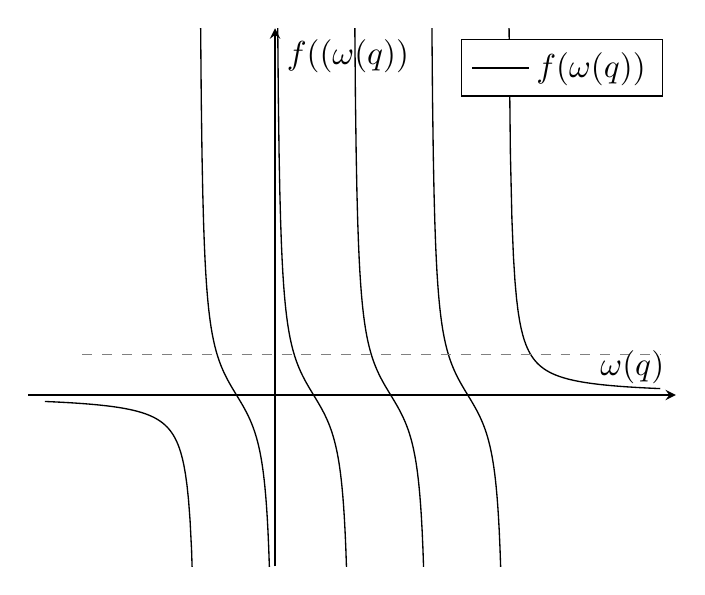
\begin{tikzpicture}[scale=1.2]
\begin{axis}[
    axis lines=middle,
    ticks=none,
    xmin=-2.5*pi,xmax=4.5*pi,ymin=-pi,ymax=8,
    xlabel={$\omega(q)$},
    ylabel={$f(\qty(\omega(q))$},
    domain=-10000:10000,
    restrict y to domain=-100000:100000,
    enlargelimits=true
    ]
% parts:
\addplot[black,domain=-3.1-2*pi:-0.01-pi,unbounded coords=jump,samples=101] {1/(x+pi)};
\addplot[black,domain=-3.1:-0.01,unbounded coords=jump,samples=101] {cot(deg(x))};
\addplot[black,domain=-3.1+pi:-0.01+pi,unbounded coords=jump,samples=101] {cot(deg(x))};
\addplot[black,domain=-3.1+2*pi:-0.01+2*pi,unbounded coords=jump,samples=101] {cot(deg(x))};
\addplot[black,domain=-3.1+3*pi:-0.01+3*pi,unbounded coords=jump,samples=101] {cot(deg(x))};
\addplot[black,domain=-3.1+4*pi:-0.01+5*pi,unbounded coords=jump,samples=101] {1/(x-3*pi)};

\addplot[dashed, black!50!white,domain=-2.5*pi:5*pi] {1};
\addlegendentry{$f\qty(\omega(q))$}
\end{axis}
\end{tikzpicture}
\end{figure}
\end{solution}

\begin{exercise}
Show that the solution for the expansion coefficients is given by
\begin{equation}\label{eq:435}
    \phi_k(q) = \dfrac{V_q}{\omega(q) - (\varepsilon_{k+q}-\varepsilon_{k})}
\end{equation}
\end{exercise}

\begin{solution}
Inserting the solution given above, \eqref{eq:435}, in the solution of exercise 4.3.2, given in \eqref{eq:432}, on the LHS we get
\begin{equation}
\begin{split}
    \phi_{k}(q) &= \dfrac{V_q}{\omega(q) - (\varepsilon_{k+q}-\varepsilon_k)}\sum_{k'}(f_{k'} - f_{k'+q}) \phi_{k'}(q) \\&= \dfrac{V_q}{\omega(q) - (\varepsilon_{k+q}-\varepsilon_k)}\sum_{k'}V_q\dfrac{f_{k'} - f_{k'+q}}{\omega(q) - (\varepsilon_{k'+q}-\varepsilon_k')}
\end{split}
\end{equation}
The solution must satisfy the transcendental equation, \eqref{eq:433}, for a solution to exist. Hence the sum over $k'$ must equal 1 and consequently the remaining term is the ansatz.
\end{solution}

\begin{exercise}
Sketch the form of this function and compare with the corresponding result for the finite system.
\begin{equation}
    \text{r.h.s. of Eq. (19)} = \mathrm{Re}\{\epsilon(q, \omega)\} \approx 1 - \dfrac{\alpha(q)}{\omega - (\langle\varepsilon_{k+q} - \varepsilon_{k}\rangle) + \gamma}
\end{equation}
where $\langle\varepsilon_{k+q} - \varepsilon_{k}\rangle$ denotes the average of the allowed non-interacting transition energies and $\gamma$ is a positive number.
\end{exercise}
\begin{solution}
As with the previous expression (Look in problem handout) we look for the case when the real part of the dielectric function vanishes, this is the case when
\begin{equation}
    1 = \frac{\alpha(q)}{\omega - \langle (\varepsilon_{k+q} - \varepsilon_k) \rangle + \gamma}
\end{equation}
This equation is sketched below:
\begin{figure}[h!]
\centering
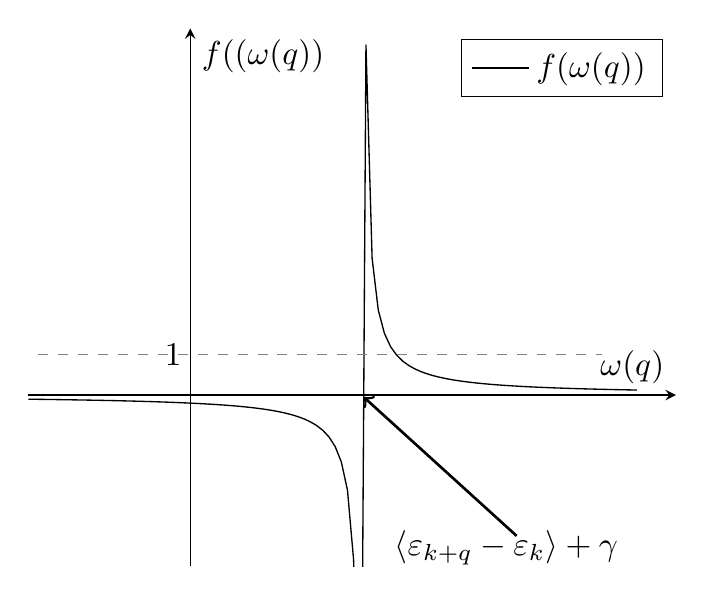
\begin{tikzpicture}[scale=1.2]
\begin{axis}[
    axis lines=middle,
    ticks=none,
    xmin=-1*pi,xmax=4*pi,ymin=-pi,ymax=8,
    xlabel={$\omega(q)$},
    ylabel={$f(\qty(\omega(q))$},
    domain=-10000:10000,
    restrict y to domain=-100000:100000,
    enlargelimits=true
    ]
% parts:
\addplot[black,domain=-5.1:13 ,unbounded coords=jump,samples=102] {1/(x-5)};
\node at (-0.5,1) {1};

\addplot[dashed, black!50!white,domain=-5:12] {1};
\addlegendentry{$f\qty(\omega(q))$}
\draw[->, thick] (9.5,-3.5) -- (5.05,-0.05);
\node at (9.2,-3.8) {$\langle \varepsilon_{k+q} - \varepsilon_k \rangle + \gamma$};
\end{axis}
\end{tikzpicture}
\end{figure}
\end{solution}
